% Options for packages loaded elsewhere
\PassOptionsToPackage{unicode}{hyperref}
\PassOptionsToPackage{hyphens}{url}
\PassOptionsToPackage{dvipsnames,svgnames,x11names}{xcolor}
%
\documentclass[
  12pt,
  a4paper,
  12pt]{article}

\usepackage{amsmath,amssymb}
\usepackage{setspace}
\usepackage{iftex}
\ifPDFTeX
  \usepackage[T1]{fontenc}
  \usepackage[utf8]{inputenc}
  \usepackage{textcomp} % provide euro and other symbols
\else % if luatex or xetex
  \usepackage{unicode-math}
  \defaultfontfeatures{Scale=MatchLowercase}
  \defaultfontfeatures[\rmfamily]{Ligatures=TeX,Scale=1}
\fi
\usepackage{lmodern}
\ifPDFTeX\else  
    % xetex/luatex font selection
  \setmainfont[]{Times New Roman}
\fi
% Use upquote if available, for straight quotes in verbatim environments
\IfFileExists{upquote.sty}{\usepackage{upquote}}{}
\IfFileExists{microtype.sty}{% use microtype if available
  \usepackage[]{microtype}
  \UseMicrotypeSet[protrusion]{basicmath} % disable protrusion for tt fonts
}{}
\usepackage{xcolor}
\setlength{\emergencystretch}{3em} % prevent overfull lines
\setcounter{secnumdepth}{5}
% Make \paragraph and \subparagraph free-standing
\ifx\paragraph\undefined\else
  \let\oldparagraph\paragraph
  \renewcommand{\paragraph}[1]{\oldparagraph{#1}\mbox{}}
\fi
\ifx\subparagraph\undefined\else
  \let\oldsubparagraph\subparagraph
  \renewcommand{\subparagraph}[1]{\oldsubparagraph{#1}\mbox{}}
\fi


\providecommand{\tightlist}{%
  \setlength{\itemsep}{0pt}\setlength{\parskip}{0pt}}\usepackage{longtable,booktabs,array}
\usepackage{calc} % for calculating minipage widths
% Correct order of tables after \paragraph or \subparagraph
\usepackage{etoolbox}
\makeatletter
\patchcmd\longtable{\par}{\if@noskipsec\mbox{}\fi\par}{}{}
\makeatother
% Allow footnotes in longtable head/foot
\IfFileExists{footnotehyper.sty}{\usepackage{footnotehyper}}{\usepackage{footnote}}
\makesavenoteenv{longtable}
\usepackage{graphicx}
\makeatletter
\def\maxwidth{\ifdim\Gin@nat@width>\linewidth\linewidth\else\Gin@nat@width\fi}
\def\maxheight{\ifdim\Gin@nat@height>\textheight\textheight\else\Gin@nat@height\fi}
\makeatother
% Scale images if necessary, so that they will not overflow the page
% margins by default, and it is still possible to overwrite the defaults
% using explicit options in \includegraphics[width, height, ...]{}
\setkeys{Gin}{width=\maxwidth,height=\maxheight,keepaspectratio}
% Set default figure placement to htbp
\makeatletter
\def\fps@figure{htbp}
\makeatother

\addtolength{\oddsidemargin}{-.5in}%
\addtolength{\evensidemargin}{-1in}%
\addtolength{\textwidth}{1in}%
\addtolength{\textheight}{1.7in}%
\addtolength{\topmargin}{-1in}%
\makeatletter
\makeatother
\makeatletter
\makeatother
\makeatletter
\@ifpackageloaded{caption}{}{\usepackage{caption}}
\AtBeginDocument{%
\ifdefined\contentsname
  \renewcommand*\contentsname{Table of contents}
\else
  \newcommand\contentsname{Table of contents}
\fi
\ifdefined\listfigurename
  \renewcommand*\listfigurename{List of Figures}
\else
  \newcommand\listfigurename{List of Figures}
\fi
\ifdefined\listtablename
  \renewcommand*\listtablename{List of Tables}
\else
  \newcommand\listtablename{List of Tables}
\fi
\ifdefined\figurename
  \renewcommand*\figurename{Figure}
\else
  \newcommand\figurename{Figure}
\fi
\ifdefined\tablename
  \renewcommand*\tablename{Table}
\else
  \newcommand\tablename{Table}
\fi
}
\@ifpackageloaded{float}{}{\usepackage{float}}
\floatstyle{ruled}
\@ifundefined{c@chapter}{\newfloat{codelisting}{h}{lop}}{\newfloat{codelisting}{h}{lop}[chapter]}
\floatname{codelisting}{Listing}
\newcommand*\listoflistings{\listof{codelisting}{List of Listings}}
\makeatother
\makeatletter
\@ifpackageloaded{caption}{}{\usepackage{caption}}
\@ifpackageloaded{subcaption}{}{\usepackage{subcaption}}
\makeatother
\makeatletter
\@ifpackageloaded{tcolorbox}{}{\usepackage[skins,breakable]{tcolorbox}}
\makeatother
\makeatletter
\@ifundefined{shadecolor}{\definecolor{shadecolor}{rgb}{.97, .97, .97}}
\makeatother
\makeatletter
\makeatother
\makeatletter
\makeatother
\ifLuaTeX
  \usepackage{selnolig}  % disable illegal ligatures
\fi
\usepackage[]{natbib}
\bibliographystyle{agsm}
\IfFileExists{bookmark.sty}{\usepackage{bookmark}}{\usepackage{hyperref}}
\IfFileExists{xurl.sty}{\usepackage{xurl}}{} % add URL line breaks if available
\urlstyle{same} % disable monospaced font for URLs
\hypersetup{
  pdftitle={Political Leadership Survival in the Aftermath of Coups and Overstays: From Illegitimate Ascent to Unexpected Exit},
  pdfauthor={Zhu Qi},
  pdfkeywords={Political survival, Coups, Overstays},
  colorlinks=true,
  linkcolor={blue},
  filecolor={Maroon},
  citecolor={Blue},
  urlcolor={Blue},
  pdfcreator={LaTeX via pandoc}}


\begin{document}


\def\spacingset#1{\renewcommand{\baselinestretch}%
{#1}\small\normalsize} \spacingset{1}


%%%%%%%%%%%%%%%%%%%%%%%%%%%%%%%%%%%%%%%%%%%%%%%%%%%%%%%%%%%%%%%%%%%%%%%%%%%%%%

\date{December 17, 2023}
\title{\bf Political Leadership Survival in the Aftermath of Coups and
Overstays: From Illegitimate Ascent to Unexpected Exit}
\author{
Zhu Qi\\
Department of Government, University of Essex\\
}
\maketitle

\bigskip
\bigskip
\begin{abstract}
This paper delves into the duration of political leaders' tenures,
focusing on two specific categories: leaders who come into power through
coups and those who exceed their designated term limits. It argues that
the length of political leadership tenures is not solely determined by
their governing strategies but also by the means through which they
ascend to power. By employing a survival model, this study demonstrates
that leaders who surpass their term limits generally have longer tenures
compared to those entering through coups.
\end{abstract}

\noindent%
{\it Keywords:} Political survival, Coups, Overstays
\vfill

\newpage
\spacingset{1.9} % DON'T change the spacing!
\ifdefined\Shaded\renewenvironment{Shaded}{\begin{tcolorbox}[sharp corners, interior hidden, breakable, frame hidden, boxrule=0pt, borderline west={3pt}{0pt}{shadecolor}, enhanced]}{\end{tcolorbox}}\fi

\setstretch{1.75}
\hypertarget{introduction}{%
\section{Introduction}\label{introduction}}

The investigation into the enduring tenure of certain leaders compared
to those with briefer terms has remained a focal point within the realm
of political science. This probing inquiry has garnered extensive
attention and undergone thorough analysis across numerous scholarly
works, as highlighted in Chapter 2.

Prior research examining the longevity of political leaders has
highlighted two prominent features. Firstly, scholars have primarily
concentrated on general frameworks that encompass either all regime
types or all autocracies, dedicating less attention to the exploration
of specific leader profiles. Secondly, existing studies have
predominantly revolved around analyzing the probability of irregular
leader exits using country-year data, leaving a void in discussions
regarding the duration of leadership tenures based on comprehensive
duration data.

Due to these significant gaps, this paper aims to conduct a comparative
analysis between two specific types of political leaders: those who rise
to power through coups and those who exceed their designated term
limits. Examining the tenures of these two irregularly ascended leaders
holds particular significance for two reasons.

Firstly, irregularly ascended leaders constitute the majority of
irregular exits from power. According to \citep{goemans2009}, between
1945 and 2015, among 1472 leaders who assumed office through regular
channels, around 213 exited irregularly (about 14.5\%). Conversely, out
of 308 leaders who assumed office through irregular means, roughly 158
(about 51.3\%) experienced irregular exits. Secondly, among irregularly
ascended leaders, the majority gained power through coups or overstays.
As per \citep{goemans2009}, out of 374 leaders who exited irregularly,
246 were ousted through coups, constituting 65.8\% of these cases.
Accordingly, there are 246 coup-entry leaders. Moreover, between 1945
and 2020, there were 106 attempts to overstay in power, of which 86 were
successful. This overstaying, detailed in ``Determinants of Incumbent
Overstay Attempts and Outcomes,'' can be perceived as a form of
self-coup, as incumbents orchestrate tactics to prolong their rule,
effectively staging coups against potential future leaders. Hence, it
becomes both relevant and enlightening to delve into and compare the
tenures of survival between coup-entry leaders and overstaying
(self-coup) leaders.

However, while existing research extensively delves into the factors
leading to coups or overstays, there remains a crucial need for more
attention directed towards what occurs after these irregular ascents.
Specifically, how do leaders' methods of entering power affect not only
their subsequent tenures but also their departures from power? This
study proposes that the manner in which leaders ascend to power
significantly impacts the duration of their leadership tenure. Unlike
leaders who overstay, those who enter through coups face more
substantial challenges concerning legitimacy, uncertainty, instability,
and power-sharing, potentially diminishing their survival duration.
Employing a survival model, this paper suggests that leaders who
overstay their term limits generally enjoy longer tenures compared to
those who gain power through coups.

This study could offer dual contributions. First, it emphasizes that the
duration of survival and unexpected exits is not solely dictated by
leaders' conduct after assuming power but is fundamentally shaped by
their methods of gaining power. It accentuates a significant difference
in tenures between overstaying leaders and coup-entry leaders. Second,
it provides empirical measurements to compare the tenure duration of
these two irregularly ascended leaders, offering insights into their
distinct impacts on the longevity of leadership.

After the introduction, the second section encompasses a comprehensive
literature review on political survival and highlighting the
contributions of this paper might offer. The third chapter delves into
the examination of factors influencing the survival of leaders who have
ascended to power through unconstitutional means. Chapter 4 provides an
account of the methodology and data employed, utilizing a survival model
for a comprehensive analysis of the determinants of leaders' survival.
Chapter 5 presents the findings of this analysis, facilitating an
in-depth discussion of the results. Finally, in Chapter 6, the paper
concludes by synthesizing these findings and exploring their broader
implications.

\hypertarget{literature-review-the-dynamics-of-leadership-survival-in-different-scenarios}{%
\section{Literature review: The dynamics of leadership survival in
different
scenarios}\label{literature-review-the-dynamics-of-leadership-survival-in-different-scenarios}}

In their seminal work, \citet{buenodemesquita2003} conducted a
comprehensive examination of leaders spanning diverse political
landscapes, encompassing democracies and autocracies, as well as
parliamentary and presidential systems, while accounting for both
civilian and military contexts. Their aim was to provide an general
explanation for the dynamics of political leadership survival within a
universal framework. Proposing a universal theoretical framework
regarding the political survival is highly intriguing. However, it is
crucial to acknowledge the challenges that must be addressed in order to
provide a more general theory of leadership survival across all types of
regimes.

Within democratic systems, there are apparent distinctions between
parliamentary and presidential regimes. In parliamentary countries like
the UK and Japan, political parties may retain power for extended
periods despite frequent changes in prime ministership. An instance of
this occurred in the UK in 2022, witnessing three different prime
ministers while the Conservative Party remained in power. Conversely, in
presidential countries such as the United States, leaders serve fixed
terms, resulting in more regular and predictable power transitions. The
spectrum of autocratic regimes is even more diverse, each characterized
by distinct features, including civilian autocracy, personnel autocracy,
military regimes, party dominance, and monarchies. Some regimes strictly
adhere to periodic power transitions, as seen in autocratic Mexico from
1919 to 2000, where each president served a fixed six-year term without
facing overthrows or overstays \citep{klesner2019}. Additionally, there
are instances where dictators rule indefinitely, passing power to their
sons, such as in Syria and North Korea, or to brothers, as observed in
Cuba. However, there are also numerous cases where rulers are ousted
unexpectedly.

Furthermore, the division of residents into different coalitions or
groups may not hold as much relevance in democracies when compared to
autocracies. In democratic systems, while those who support and vote for
incumbents may witness their advocated policies enacted, those opposing
them still experience the same policies. For instance, if a candidate
advocating for lower taxes wins an election, it doesn't lead to lower
taxes for the candidate's supporters and higher taxes for their
opponents; both groups encounter identical tax levels. This dynamic
differs significantly in autocratic regimes, where distinct groups
benefit unequally based on their status and relationships with the
rulers.

Moreover, the rules governing power transitions differ drastically
between democracies and autocracies. In most autocratic regimes, the
process of leadership selection remains shrouded in secrecy. Expressing
dissenting views, whether as potential challengers or supporters of
challengers, can be perilous. In Russia, despite the presence of general
elections, challengers frequently face severe consequences such as
assassination, poisoning, imprisonment, or exile. Due to the lack of
transparent and fair conventional procedures for power transitions, it's
challenging to assess who holds more power or has more supporters. A
dictator could potentially survive a lengthy tenure despite weak support
because the true balance of power remains undisclosed. Conversely, a
powerful ruler could be ousted by a small number of guards because the
army or other supporters hesitate to fight for them due to a lack of
information regarding their predominant status in the power balance.
Thus, accurately calculating selectorates or coalitions, as
\citet{buenodemesquita2003} did in their research, becomes impossible in
such scenarios. In contrast, in democracies, challengers can openly vie
for leadership without fear. Their support rates are easily discernible,
and they can seek to gain more supporters through public speeches, TV or
newspaper advertisements, or assemblies. If their support rates are not
adequate to challenge the incumbents, different groups can try to
collaborate, facilitating power transitions with a slightly higher level
of support.

Given the distinct nature of political leadership survival in various
regimes, scholars have increasingly focused on understanding the
survival dynamics specific to certain regime types, such as democracies
\citep{svolik2014} and autocracies \citep{davenport2021}. Notably,
considerable academic attention has been drawn towards unexpected
tenures, particularly those leaders who either fail to complete their
original terms or overstay their terms. Scholars have predominantly
revolved around two primary dimensions. The first dimension encompasses
contextual conditions and resources available to leaders. These factors
include elements such as the leaders' personal competence
\citep{yu2016}, societal stability \citep{arriola2009}, economic
development level \citep{palmer1999, williams2011}, access to natural
resources \citep{smith2004, quirozflores2012}, and external support
networks \citep{licht2009, wright2008, thyne2017}. The second dimension
delves into the strategies implemented by leaders in enacting their
political and economic policies. This includes their responses to
challengers and dissent within their regimes
\citep{escribà-folch2013, davenport2021}, as well as strategies used in
policy-making \citep{gandhi2007, morrison2009}.

Unsurprisingly, a considerable focus in previous studies has been
directed towards coups, given their status as a prominent pathway
leading to the exit of authoritarian leaders
\citep{svolik2008, frantz2016}. Literature on leadership survival has
examined strategies aimed at preventing coups
\citep{powell2017, sudduth2017, debruin2020}, as well as analyses of how
leaders extend their tenures post-surviving failed coup attempts
\citep{easton2018}. For instance, \citet{sudduth2017a}, while primarily
focused on purge strategies, examines the post-coup actions of a
dictator. The central argument suggests that leaders ascending through
coups experience a temporary surge in influence compared to elites
immediately following the coups, making them less prone to subsequent
ousting by coup attempts. This argument challenges the traditional
notion that new leaders are generally in a weak position at the start of
their tenure \citep{roessler2011}. Despite this distinction, both
Sudduth and prior scholars concur that new leaders tend to purge rival
elite groups to consolidate their power. However, Sudduth argues that
dictators undertake purges when they can do so without significant risk,
while traditional views suggest purges occur when dictators perceive
imminent threats. However, it's imperative to acknowledge that new
leaders, particularly those ascending through unconventional means,
don't adhere to a universal pattern of inherent weakness or strength.
Leadership transitions unfold in varied contexts, presenting leaders
with diverse challenges.

Scholars have extensively scrutinized the resilience of political
leaders across diverse realms, encompassing universal frameworks,
autocratic regimes, and the aftermath of failed challenges, such as coup
attempts. Interestingly, there has been limited discourse concerning the
survival dynamics of leaders who manage to maintain power following
successful coups or prolonged incumbency. This study endeavors to bridge
this gap by specifically scrutinizing and delineating the survival
duration between these two categories of leaders.

\hypertarget{the-logic-of-political-leader-survival-in-irregular-ascensions}{%
\section{The logic of political leader survival in irregular
ascensions}\label{the-logic-of-political-leader-survival-in-irregular-ascensions}}

Engaging in a discourse on the survival strategies of political leaders
within non-democratic regimes presents a significant challenge. The
complexity stems from the lack of a universal pattern that encapsulates
the rules or conventions dictating power transitions in autocratic
systems. For instance, even in Middle Eastern monarchies, the transfer
of power doesn't rigidly adhere to a father-to-son lineage. However,
this doesn't imply that analyzing survival strategies in autocracies is
unattainable. Despite substantial differences, they share certain
commonalities. Most autocratic regimes, especially those characterized
by irregular ascensions, exhibit three prevalent situations.

The first aspect concerns the issue of legitimacy. Leaders who ascend
through coups lack legitimacy as they seize power through force or other
unconventional means. While many leaders prolong their tenures through a
façade of constitutional procedures, such as judgments by the Supreme
Court, congressional votes, or even referendums, they often manipulate
these processes to maintain control. It's commonly understood by ruling
elites, opposition parties, and the populace that these leaders lack
legitimacy. This lack of legitimacy can sometimes justify the cause of
those seeking their replacement, even if the means used are
unconstitutional.

The second characteristic revolves around the uncertainty surrounding
power transitions. This uncertainty creates ambiguity not only for
ruling elites and ordinary citizens but also for the leaders themselves
regarding when, how, and to whom power might be transferred. Such
uncertainty breeds inherent instability. Amidst such instability, people
experience a lack of security. This perception often leads to the belief
that the current ruler is incompetent and should be replaced by someone
more powerful or capable. Consequently, the ruling elite or opposition
factions may exploit the instability as an opportunity to challenge
existing power structures.

The third aspect revolves around the equilibrium of power. In
autocracies, governance typically rests with a minority faction that
possesses a highly structured organization, distinctly contrasting with
the decentralized and disorganized subjects. Even amid protests or
uprisings, ruling groups adeptly suppress such incidents individually.
The possibility of overthrowing tyranny arises if the subjects can
coalesce their efforts. However, the principal obstacle lies in the
formidable challenge of surmounting the collective action problem.
Autocratic dictators commonly adopt a ruling strategy focused on
preventing unity among subjects and complicating endeavors to address
collective action issues. This elucidates why dictatorships curtail free
expression, assembly, and association. The absence of free public
expression and association renders the power balance unclear.
Consequently, rulers maintain relative power advantages over not only
the elites but also the subjects.

The trifecta of illegitimacy, uncertainty, and the equilibrium of power
profoundly impact the longevity of a regime. Yet, compared to leaders
who gain power through coups, those who overstay their terms find
themselves in a comparatively advantageous position concerning these
three aspects.

\hypertarget{legitimacy}{%
\subsection{Legitimacy}\label{legitimacy}}

As per Powell and Thyne's definition, coups constitute ``illegal and
overt attempts by the military or other elites within the state
apparatus to unseat the sitting executive.'' \citep[p.252]{powell2011}.
While it is undeniable that a few coups have been justified by resolving
crises and leading to improved outcomes, they remain illegal means to
remove incumbents. These unlawful methods open Pandora's box, publicly
suggesting alternatives to constitutional procedures for seizing power,
particularly in the case of successful coups. Such actions inevitably
prompt imitators to launch new coups. As society becomes accustomed to
coups, subsequent ones may not elicit significant backlash, given that
the incumbents themselves ascended to power through similar means.
Furthermore, coups not only invite further coups but also embolden
external challengers, including uprisings, revolutions, and civil wars
\citep{dahl2023}.

On the other hand, leaders who overstay their tenures may lack
legitimacy but often manage to maintain power through a facade of
legitimacy. They don't blatantly seize power via military force but
rather cling to power through parliamentary or congressional processes,
the Supreme Court, and even nationwide referendums. The opposition
usually chooses to confront these leaders using legal means, engaging in
legislative debates or legal proceedings, and sometimes by advocating
for another referendum. Attempts to overthrow leaders who overstay their
terms through coups would be even less legitimate and might struggle to
garner support. However, removing such leaders within the boundaries of
the law presents an arduous challenge, if not a near-impossible task.

\hypertarget{uncertainty}{%
\subsection{Uncertainty}\label{uncertainty}}

As previously discussed, both leaders who assume power through coups and
those who extend their terms contribute to uncertainties within their
regimes. However, regimes led by overstaying rulers generally
demonstrate lesser overall uncertainty.

Primarily, following coups, regimes face uncertainty regarding four
potential outcomes: democracies initially overthrown by coups may either
persist as democracies (I) or transition into autocracies (II), while
autocracies overthrown by coups may either endure as autocracies (III)
or evolve into democracies (IV). In contrast, regimes with leaders
overstaying their terms, with only rare exceptions, typically persist as
autocracies.

Secondly, the anticipated duration of future ruling tenures tends to be
longer for overstaying rulers than for coup-entry leaders. Most
overstaying leaders endeavor to prolong their tenures for as long as
possible. For example, figures like Putin in Russia and Xi Jinping in
China are less inclined to voluntarily step down unless forcibly removed
from power. Conversely, coup-entry leaders face greater uncertainty.
Coups are often justified through diverse excuses or claims. Some assert
their actions as defending democratic order, exemplified by President
Manuel Zelaya's ousting in Honduras in 2009. Others claim to protect the
constitution, such as President Mamadou Tandja's overthrow in Niger in
2010. The complexity arises when certain coup leaders honor their
promises by transferring power to a constitutional successor. For
instance, following the 2010 coup in Niger, a new constitution restored
civilian power and reinstated a strict two-term limit on the presidency
in the same year \citep{ginsburg2019}. However, numerous others refuse
to step down and retain power, as observed in the 1973 coup in Chile
\citep{ökten2022}.

Thirdly, uncertainties abound regarding policy changes and power
reshuffling. Comparatively, coup-entry leaders need to restructure top
officials and justify their actions by implementing noticeable
differences after overthrowing the incumbents. In contrast, overstaying
leaders face fewer issues as their regimes experience minimal dramatic
changes. There is no rush to dismantle the old ruling paradigm and
establish a new order.

\hypertarget{equilibrium-of-power}{%
\subsection{Equilibrium of power}\label{equilibrium-of-power}}

Rulers in autocracies face a challenging dilemma in managing powerful
elites. They require a strong force to counter potential external
threats while constantly grappling with the fear of being replaced by
competent and ambitious subordinates. Therefore, maintaining a delicate
balance of power becomes a sophisticated skill. It's apparent that
sustaining equilibrium is easier than restoring it once disrupted.

In regimes with leaders overstaying their terms, there exists, at least
temporarily, a superficial equilibrium of power. Successful overstays
demonstrate the incumbents' firm grip on power, effectively deterring
both internal dissent and external challenges. Consequently, this
contributes to the overall stability of the governing structure and
society.

Conversely, leaders who come to power through coups invariably disrupt
the balance of power and must establish a new equilibrium, even in
relatively peaceful coup scenarios. The overthrow of previous rulers
necessitates the dismantling of the existing ruling framework and a
reshuffling of top officers and officials. These actions inevitably
breed turbulence and adversaries for the new rulers, making the
restoration of order and the balance of power considerably more
challenging.

Internal conflicts among elites, as highlighted by numerous scholars,
pose a significant threat to the stability of those in power. Hence,
they are often compelled to negotiate and compromise among external
factions. As noted by \citet{roessler2011}, these rulers might attempt
to reduce the likelihood of subsequent coups, albeit at the expense of
increasing the risk of societal rebellions and civil wars. This strategy
resonates with the approach adopted by Chinese leader Chiang Kai-shek in
the 1930s. He pursued a strategy of compromise with both Japan and the
Soviet Union to eliminate the internal threat posed by the Chinese
Communist Party, prioritizing ``Domestic stability takes precedence over
resisting foreign invasion'' during that period \citep{chu1999chiang}.
However, adopting a hardline stance internally could not only weaken
themselves by purging elites, but also incite backlash from close
allies, as witnessed in instances like Idi Amin's coup in 1971 in Uganda
and Pervez Musharraf's coup in 1999 in Pakistan \citep{sudduth2017a}.

These factors collectively contribute to a shorter expected lifespan of
regimes following coups \citep{dahl2023}, compared to relatively longer
tenures for overstaying regimes. Analyzing a comprehensive coup dataset
\citep{powell2011} spanning from 1950 to 2023, it's evident that 97
countries experienced coups during this period. Among them, 15 countries
endured at least 10 coups, and 10 countries witnessed more than 6
successful coups, reinforcing the analysis discussed above.

Based on a log-rank test in survival analysis, see
Figure~\ref{fig-logrank} using the leaders dataset \citep{goemans2009}
in conjunction with the author's incumbent overstay dataset, a clear
trend emerges: leaders who overstay their incumbency exhibit
significantly longer survival rates compared to those who enter through
coups. Specifically, the average survival time \textbf{after}
overstaying, discounting their original term time, is approximately 10.1
years. In contrast, coup-entry leaders tend to have an average survival
time of 4.1 years.

\begin{figure}

{\centering 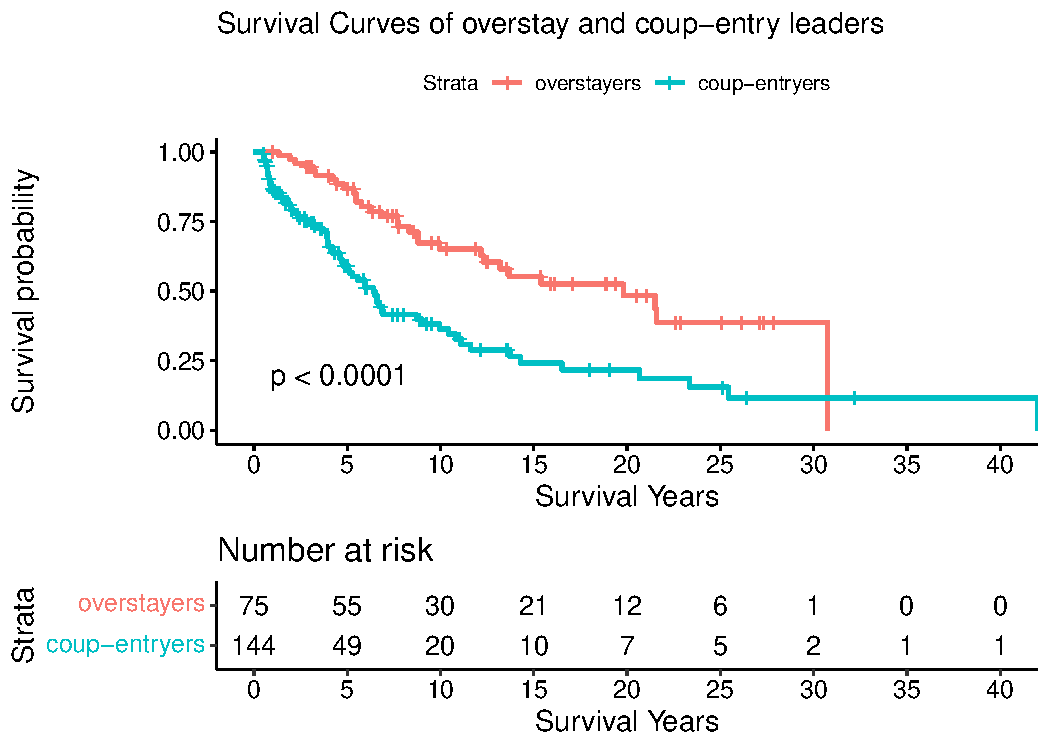
\includegraphics{survival_after_coups_jasa_files/figure-pdf/fig-logrank-1.pdf}

}

\caption{\label{fig-logrank}Kaplan-Meier plot}

\end{figure}

Based on these insights, I propose the following hypothesis:

\textbf{Hypothesis:} Political leaders who successfully extend their
time in power are more likely to have prolonged survival compared to
leaders who assume power through coups.

In the upcoming section, I'll outline the research methodology employed
in this paper. The goal is to delve deeply into understanding the
factors influencing the survival duration of incumbent overstaying
leaders and coup-entry leaders. This investigation aims to elucidate the
extent to which these identified factors impact the survival durations
of these distinct groups.

\hypertarget{method-and-data}{%
\section{Method and data}\label{method-and-data}}

\newpage


\renewcommand\refname{References}
  \bibliography{survival.bib}


\end{document}
